\documentclass[14pt]{beamer}
\usepackage{./Estilos/BeamerUVM}
\usepackage{./Estilos/ColoresLatex}
\usepackage{circuitikz}
\usepackage{schemata}
\usetheme{Warsaw}
\usecolortheme{rose}
%\useoutertheme{default}
\setbeamercovered{invisible}
% or whatever (possibly just delete it)
\setbeamertemplate{section in toc}[sections numbered]
\setbeamertemplate{subsection in toc}[subsections numbered]
\setbeamertemplate{subsection in toc}{\leavevmode\leftskip=3.2em\rlap{\hskip-2em\inserttocsectionnumber.\inserttocsubsectionnumber}\inserttocsubsection\par}
%\setbeamercolor{section in toc}{fg=blue}
%\setbeamercolor{subsection in toc}{fg=blue}
%\setbeamercolor{frametitle}{fg=blue}
\setbeamertemplate{caption}[numbered]

\setbeamertemplate{footline}
\beamertemplatenavigationsymbolsempty
\setbeamertemplate{headline}{}


\makeatletter
\setbeamercolor{section in foot}{bg=gray!30, fg=black!90!orange}
\setbeamercolor{subsection in foot}{bg=blue!30}
\setbeamercolor{date in foot}{bg=black}
\setbeamertemplate{footline}
{
  \leavevmode%
  \hbox{%
  \begin{beamercolorbox}[wd=.333333\paperwidth,ht=2.25ex,dp=1ex,center]{section in foot}%
    \usebeamerfont{section in foot} \insertsection
  \end{beamercolorbox}%
  \begin{beamercolorbox}[wd=.333333\paperwidth,ht=2.25ex,dp=1ex,center]{subsection in foot}%
    \usebeamerfont{subsection in foot}  \insertsubsection
  \end{beamercolorbox}%
  \begin{beamercolorbox}[wd=.333333\paperwidth,ht=2.25ex,dp=1ex,right]{date in head/foot}%
    \usebeamerfont{date in head/foot} \hspace*{2em}
    \insertframenumber{} / \inserttotalframenumber \hspace*{2ex} 
  \end{beamercolorbox}}%
  \vskip0pt%
}
\makeatother

\makeatletter
\patchcmd{\beamer@sectionintoc}{\vskip1.5em}{\vskip0.8em}{}{}
\makeatother
% \usefonttheme{serif}
\usepackage[clock]{ifsym}
\DeclareSIUnit\erg{erg}
\DeclareSIUnit[number-unit-product = {\,}]\cal{cal}

\sisetup{per-mode=symbol}
\resetcounteronoverlays{saveenumi}

% Macro para agregar el logo de UVM en cada slide de la presentación

\addtobeamertemplate{frametitle}{}{%
\begin{tikzpicture}[remember picture,overlay]
\coordinate (logo) at ([xshift=-1.5cm,yshift=-0.8cm]current page.north east);
% \fill[devryblue] (logo) circle (.9cm);
% \clip (logo) circle (.75cm);
\node at (logo) {
\includegraphics[width=2.1cm]{Imagenes/logo_UVM.png}};
\end{tikzpicture}}


\title{\Large{Potencial de acción} \\ \normalsize{Física IV (Área II)}}
\date{}

\begin{document}
\maketitle

\section*{Contenido}
\frame[allowframebreaks]{\frametitle{Contenido} \tableofcontents[currentsection, hideallsubsections]}


\section{El potencial de equilibrio}
\frame{\tableofcontents[currentsection, hideothersubsections]}
\subsection{}

\begin{frame}
\frametitle{¿Qué es el potencial de equilibrio?}
Toda célula está delimitada por una membrana plasmática formada por una bicapa de lípidos, lo que le confiere un carácter \textocolor{byzantine}{hidrofóbico}.
\end{frame}
\begin{frame}
\frametitle{Permeabilidad de la membrana}
No obstante, la membrana es semipermeable a una amplia variedad de moléculas, \pause lo que resulta en una diferencia en la composición del citoplasma y el medio extracelular.
\end{frame}
\begin{frame}
\frametitle{Permeabilidad de la membrana}
De entre todas las moléculas, \pause los iones resultan ser de vital importancia para múltiples funciones celulares.
\end{frame}
\begin{frame}
\frametitle{¿Qué es un ion?}
Un ion es un átomo o molécula que \textocolor{burgundy}{ha ganado} o \textocolor{carmine}{perdido} uno o más electrones, lo que resulta en una carga eléctrica neta.
\end{frame}
\begin{frame}
\frametitle{¿Qué es un ion?}
Esta carga eléctrica puede ser positiva si el ion ha \textocolor{cerulean}{perdido electrones} (llamado \textocolor{cerulean}{catión}) \pause o negativa si ha \textocolor{coralred}{ganado electrones} (llamado \textocolor{coralred}{anión}).
\end{frame}
\begin{frame}
\frametitle{Permeabilidad de la membrana}
Los más abundantes son el Na+, K+, Ca2+ y Cl-, cuyos valores fisiológicos en el humano se indican en la siguiente tabla.
\end{frame}
\begin{frame}
\frametitle{Iones en el cuerpo humano}
\vspace*{-0.5cm}
\begin{table}
    \centering
    \begin{tabular}{l | c | c}
    Ion & C. intracelular & C. extracelular \\ \hline
    Na+ & 12 mM & 145 mM \\ \hline
    K+ & 155 mM & 4 mM \\ \hline
    Ca++ & 100 mM & 1.5 mM \\ \hline
    Cl- & 4.2 mM & 123 mM \\ \hline
\end{tabular}
\end{table}
\end{frame}
\begin{frame}
\frametitle{Unidades de la tabla}
Recordemos que: \textbf{mM}: \pause Milimolar, es una medida de concentración de un soluto en una disolución (\num{d-3} molar).
\end{frame}
\begin{frame}
\frametitle{Diferencia de concentraciones}
Esta diferencia en las concentraciones iónicas condiciona una \textocolor{debianred}{diferencia entre las cargas} a ambos lados de la membrana, \pause las mismas que tratarán de igualarse (\textocolor{cobalt}{equilibrio de Gibbs-Donnan}).
\end{frame}
\begin{frame}
\frametitle{Paso de iones}
Bajo ciertas condiciones, la membrana permite el paso de algunos iones, \pause lo que genera un \textocolor{red}{flujo de cargas} que depende de la permeabilidad relativa de la membrana a cada ion.
\end{frame}
\begin{frame}
\frametitle{Potencial de membrana}
Al pasar los iones a favor de su \textocolor{armygreen}{gradiente de concentración} (de donde hay más a donde hay menos) \pause se genera una \textocolor{byzantium}{diferencia de potencial eléctrico} a través de la membrana, \pause llamado \textocolor{red}{potencial de membrana} (medida en milivoltios o mV).
\end{frame}
\begin{frame}
\frametitle{Potecial de membrana}
Es de crucial importancia comprender que dicho potencial de membrana será determinado solo por las \textocolor{auburn}{concentraciones iónicas} a cada lado de la membrana \pause y por la \textocolor{bondiblue}{permeabilidad} de la misma membrana a cada ion.
\end{frame}
\begin{frame}
\frametitle{Potencial de inicio}
\vspace*{-0.75cm}
\begin{figure}
    \centering
    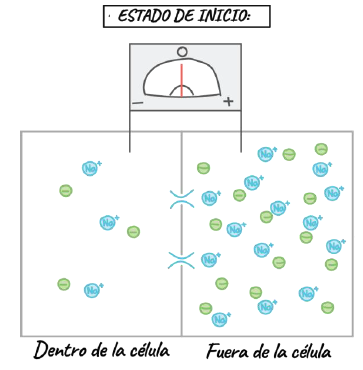
\includegraphics[scale=0.6]{Imagenes/Potencial_Accion_04.png}
\end{figure}
\end{frame}
\begin{frame}
\frametitle{Estado de inicio}
En el estadio inicial, tenemos dos compartimentos, \textocolor{ao}{adentro} y \textocolor{red}{afuera} de la célula, \pause y podemos ver que afuera de la célula hay mucho Na+ y Cl-.
\end{frame}
\begin{frame}
\frametitle{Estado de inicio}
En este caso, la membrana es \textocolor{bulgarianrose}{IMPERMEABLE} al Cl- \pause pero \textocolor{cadmiumgreen}{PERMEABLE} al Na+, \pause porque existen canales de Na que permitirán que éste difunda hacia adentro de la célula (a favor del gradiente de concentración)
\end{frame}
\begin{frame}
\frametitle{Potencial de equilibrio}
Y así el Na+,  \textocolor{cadet}{comenzará a difundir} hacia adentro de la célula.
\end{frame}
\begin{frame}
\frametitle{Potencial de equilibrio}
Pero llegará el momento en donde se \textocolor{carnelian}{detendrá su difusión} \pause porque las cargas del Cl- se encuentran atrayendo al Na+ para que regrese al medio extracelular, \pause en este momento el Na+ ha llegado a su \textocolor{ceruleanblue}{POTENCIAL DE EQUILIBRIO}.
\end{frame}
\begin{frame}
\frametitle{Potencial de equilibrio}
\vspace*{-0.75cm}
\begin{figure}
    \centering
    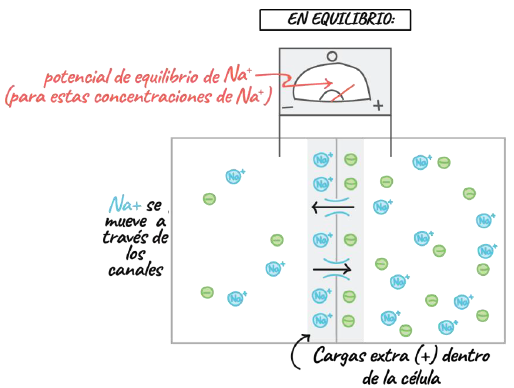
\includegraphics[scale=0.6]{Imagenes/Potencial_Accion_05.png}
\end{figure}
\end{frame}
\begin{frame}
\frametitle{Ecuación de Nerst}
Este equilibrio está descrito por la \textocolor{cinnabar}{ecuación de Nernst}, y se aplica para cada ion difusible a través de la membrana celular:
\end{frame}
\begin{frame}
\frametitle{Ecuación de Nerst}
\begin{align*}
E_{i} = \dfrac{R \, T}{z \, F} \, \ln \dfrac{\left[ \text{ion} \right]_{e}}{\left[ \text{ion} \right]_{i}}
\end{align*}
donde:
\setbeamercolor{item projected}{bg=bananayellow,fg=black}
\setbeamertemplate{enumerate items}{%
\usebeamercolor[bg]{item projected}%
\raisebox{1.5pt}{\colorbox{bg}{\color{fg}\footnotesize\insertenumlabel}}%
}
\begin{enumerate}[<+->]
\item $E_{i}$ es el potencial de equilibrio del ion X [V]
\item $R$ constante de los gases (\num{8.315} \unit{\joule\per{\kelvin\mol}})
\item $T$ temperatura en grados Kelvin
\end{enumerate}
\end{frame}

\section{El potencial de acción}
\frame{\tableofcontents[currentsection, hideothersubsections]}
\subsection{Definición}

\begin{frame}
\frametitle{¿Qué es el potencial de acción?}
El potencial de acción es un fenómeno eléctrico que ocurre en las \textocolor{ao}{células excitables}, como las neuronas y las células musculares.
\end{frame}
\begin{frame}
\frametitle{¿Qué es el potencial de acción?}
Es una \textocolor{red}{señal eléctrica rápida y temporal} \pause que se propaga a lo largo de la membrana celular y juega un papel fundamental en la comunicación celular y en la generación de respuestas específicas.
\end{frame}

\end{document}